\documentclass[12pt,a4paper]{article}
\usepackage{classeRapport} % template INSA
\usepackage{hyperref} % lien tableofcontents + url
\usepackage{graphicx} % pour les images
\usepackage{listings} % pour mettre du code
\usepackage{color} % pour la couleur dans le code
\usepackage{amsmath} % pour les matrices
\usepackage{float} % pour le [H] des figures

\hypersetup{ % couleur des liens
    colorlinks=true,
    linkcolor=black,
    filecolor=black,      
    urlcolor=blue,
}

\definecolor{backcolour}{rgb}{0.95,0.95,0.92}
 
%%%%
\definecolor{mygreen}{RGB}{28,172,0} % color values Red, Green, Blue
\definecolor{mylilas}{RGB}{170,55,241}

\lstdefinestyle{mystyle}{
    backgroundcolor=\color{backcolour},   
    basicstyle=\footnotesize,
    breakatwhitespace=false,         
    breaklines=true,                 
    captionpos=b,                    
    keepspaces=true,                 
    numbers=left,                    
    showspaces=false,                
    showstringspaces=false,
    showtabs=false,                  
    tabsize=2,
    %%%%
    language=Matlab,
    morekeywords={matlab2tikz},
    keywordstyle=\color{blue},
    morekeywords=[2]{1}, keywordstyle=[2]{\color{black}},
    identifierstyle=\color{black},
    stringstyle=\color{mylilas},
    commentstyle=\color{mygreen},
    showstringspaces=false, % without this there will be a symbol in the places where there is a space
    numberstyle={\tiny \color{black}}, % size of the numbers
    numbersep=9pt, % this defines how far the numbers are from the text
    emph=[1]{for,end,break},emphstyle=[1]\color{red}, % some words to emphasise
}

\lstset{style=mystyle}

\begin{document}

\PageDeGarde
{Images/TemplateINSA/rien} % image sur la page de garde
{Filtre de Kalman/Suivi d'objets} % titre principal
{Mini-projet TSA} % sous-titre
{Mehdi \textsc{ABOUZAID}\\
 Damien \textsc{TOOMEY}\\
 --\\
 À l'attention de \\ M. \textsc{HÉRAULT}} % nom
{TSA - ASI - 2017-2018} % bas de page

\Page{INSALogo}{rien.png} % logo de bas de page (en bas a droite)

\newpage
\tableofcontents

\newpage
\section{Étude bibliographique sur le modèle}
\subsection{Présentation} 

\indent Le filtre de Kalman est un filtre à réponse impulsionnelle infinie (RII), c’est-à-dire qu'il est basé uniquement sur les valeurs en entrée du filtre ainsi que sur les valeurs antérieures de cette même réponse. Sa fonction est donc d'estimer les états d’un système dynamique à partir d'une série de mesures incomplètes ou bruitées.

Le filtre de Kalman fait appel à la dynamique de la cible qui définit son évolution dans le temps pour obtenir de meilleures données, éliminant ainsi l'effet du bruit. Ces données peuvent être calculées pour faire du filtrage ou pour de la prédiction.

\subsection{Origine}

\indent Le filtre de Kalman a été nommé ainsi, suite à sa conception dans les années 1950 par Rudolf Kalman, mathématicien et automaticien américain d'origine hongroise. Pourtant, dès le XIX\textsuperscript{ème} siècle, Thorvald Nicolai Thiele, astronome danois, puis au XX\textsuperscript{ème} siècle, Peter Swerling, automaticien américain, avaient déjà tous les deux développé un algorithme similaire au filtre de Kalman.

\indent Stanley Schmidt est reconnu comme ayant réalisé la première mise en œuvre du filtre. C'était lors d'une visite de Rudolf Kalman à la NASA Ames Research Center qu'il vit le potentiel de son filtre pour l'estimation de la trajectoire pour le programme Apollo. Ceci a conduit à l'utilisation du filtre dans l'ordinateur de navigation.

\subsection{Fonctionnement}

\indent L'algorithme fonctionne en deux étapes, une étape de prédiction et une étape de mise à jour. La phase de prédiction utilise l'état estimé de l'instant précédent pour produire une estimation de l'état courant. Une fois les observations de l’instant courant obtenues, la seconde phase de mise à jour consiste à apporter une correction de l'état prédit dans le but d'obtenir une estimation plus précise. L'algorithme du filtre de Kalman est un processus dit récursif et markovien. Cela signifie que pour estimer l'état courant, seules l'estimation de l'état précédent et les mesures actuelles sont nécessaires, aucune autre information supplémentaire n’est requise. \\

Le filtre de Kalman est limité aux systèmes linéaires. Cependant, la plupart des systèmes physiques sont non linéaires. Le filtre n'est donc optimal que sur une petite plage linéaire des phénomènes réels. Une grande variété de filtres de Kalman a été depuis développée à partir de la formulation originale dite filtre de Kalman simple. Par exemple, Schmidt a développé le filtre de Kalman étendu, applicable aux phénomènes non linéaires. 

\paragraph{Modèles du filtre}
~~\\
\begin{itemize}
	\item[] Modèle de dynamique ou système : \\
$x_k=Ax_{k-1}+q$ \\
$x_k|x_{k-1} \sim  \mathcal{N}(x_k|Ax_{k-1},\,Q)\,$
	\item[] 
	\item[] Modèle d'observation : \\
$y_k=Hx_k+r$ \\
$y_k|x_k \sim  \mathcal{N}(y_k|Hx_k,\,R)\,$
\end{itemize}

\paragraph{Distributions des états et des observations}
~~\\
\begin{itemize}
	\item[] Pour les états : \\
	$P(x_k|y_{1:k-1}) \sim \mathcal{N}(x_k|m_k^-,\,P_k^-)\,$ \\
	$P(x_k|y_{1:k-1}) \sim \mathcal{N}(x_k|m_k^-,\,P_k^-)\,$
	\item[]
	\item[] Pour les observations : \\ 
	$P(x_k|y_{1:k-1}) \sim \mathcal{N}(x_k|m_k^-,\,P_k^-)\,$
\end{itemize}

\paragraph{Prédiction}
~~\\
\begin{itemize}
	\item[] Connaissant x[0:k-1] et y[1:k-1], on cherche à estimer x[k] : \\
	$P(x_k|y_{1:k-1}) \sim \mathcal{N}(x_k|m_k^-,\,P_k^-)\,$
	\item[] On applique le modèle de dynamique : \\
	$m_k^- = Am_{k-1}$ \\
	$P_k^- = AP_{k-1}A^T+Q$ 
\end{itemize}

\paragraph{Mise à jour} 
~~\\
\begin{itemize}
	\item[] Connaissant x[0:k-1] et y[1:k], on cherche à estimer x[k]: \\
	$P(x_k|y_{1:k}) \sim \mathcal{N}(x_k|m_k,\,P_k)\,$
	\item[] On corrige la prédiction de l'étape précédente par l'observation $k$ : \\
	$v_k=y_k-Hm_k^-$ \\
	$S_k = HP_k^-H^T+R$ \\
	$K_k = P_k^-H^TS_k^{-1}$ \\
	$m_k=m_k^-+K_kv_k$ \\
	$P_k=P_k^- - K_kS_kK_k^T$ \\
\end{itemize}

\paragraph{Détail des matrices et vecteurs}
~~\\
Nous choisissons le modèle de l'accélération constante au vu des données que avons choisies. \\

Matrice de dynamique/transfert/système
\[ A=\begin{pmatrix}
	1 & 0 & dt & 0 & 0 & 0 \\
	0 & 1 & 0 & dt & 0 & 0 \\
	0 & 0 & 1 & 0 & dt & 0 \\
	0 & 0 & 0 & 1 & 0 & dt \\
	0 & 0 & 0 & 0 & 1 & 0 \\
	0 & 0 & 0 & 0 & 0 & 1 \\
\end{pmatrix} \] 

Matrice d'observation
\[ H= \begin{pmatrix}
	1 & 0 & 0 & 0 & 0 & 0 \\
	0 & 1 & 0 & 0 & 0 & 0 \\
\end{pmatrix} \]

Vecteur d'état
\[m_k=\begin{pmatrix}
	x \\
	y \\
	\dot{x} \\
	\dot{y} \\
	\ddot{x} \\
	\ddot{y}
\end{pmatrix}\] 

Bruit de transition
\[ Q= \begin{pmatrix}
	a & 0 & 0 & 0 & 0 & 0 \\
	0 & b & 0 & 0 & 0 & 0 \\
	0 & 0 & c & 0 & 0 & 0 \\
	0 & 0 & 0 & d & 0 & 0 \\
	0 & 0 & 0 & 0 & e & 0 \\
	0 & 0 & 0 & 0 & 0 & f \\
\end{pmatrix} \quad \forall a,b,c,d,e,f \in {\rm I\!R} \]


Bruit d'observation
\[ R=\begin{pmatrix}
	g & 0 \\
	0 & h \\
\end{pmatrix} \quad \forall g,h \in {\rm I\!R} \]

Covariance de l'état initial
\[ p_0= \begin{pmatrix}
	i & 0 & 0 & 0 & 0 & 0 \\
	0 & j & 0 & 0 & 0 & 0 \\
	0 & 0 & k & 0 & 0 & 0 \\
	0 & 0 & 0 & l & 0 & 0 \\
	0 & 0 & 0 & 0 & m & 0 \\
	0 & 0 & 0 & 0 & 0 & n \\
\end{pmatrix} \quad \forall i,j,k,l,m,n \in {\rm I\!R} \]




\newpage
\section{Étude bibliographique sur l'application}
\paragraph{}
	
	Le suivi d'objet correspond au fait de localiser un objet dans une vidéo ou une séquence d'images. \\
	
	Dans les années 1960, le filtre de Kalman a été utilisé pour la première fois lors de la mission Apollo pour estimer la trajectoire de la fusée allant sur la Lune. Ce filtre est aussi utilisé pour corriger la trajectoire de missiles et calculer l'altitude d'une fusée.

	A partir des années 1990, le filtre de Kalman s'est propagé à la société civile avec les GPS\footnote{GPS : Global Positioning System} (système de positionnement global). \\

	Le filtre de Kalman permet également la fusion de données pour avoir une meilleur estimation de chaque donnée. Par exemple, si une voiture est équipée de trois capteurs :
\begin{itemize}
\item[•] système de mesure inertiel (IMU\footnote{IMU : Inertial Measurement Unit}) : mesure l'accélération et la vitesse angulaire de la voiture 
\item[•] Odomètre : donne la position relative de la voiture 
\item[•] GPS : donne la position absolue de la voiture,
\end{itemize}	 
le filtre de Kalman permet de prendre en compte les données de chaque capteur et estimer une position plus précise de la voiture. \\

	Aujourd'hui, il est possible de suivre un ou plusieurs objets dans une vidéo, en temps réel ou non, la position de la caméra étant fixe ou non. Le suivi d'objets est entre autres utilisé dans le domaine de sécurité, la réalité augmentée et le contrôle de la circulation. Si l'objet est détecté, sa position est corrigée sinon elle est prédite. \\

	Dans le cadre de notre étude, nous nous concentrerons uniquement sur le suivi d'objets (tracking). \\
\indent Vu le délai très court qui nous est imparti, nous n'étudierons le suivi d'un unique objet avec une caméra stationnaire (arrière plan constant).

\newpage
\section{Présentation du jeu de données choisi ou construit}
\subsection{Vidéo 1 : \emph{singleball.mp4}}

Pour notre projet, nous avons utilisé une vidéo nommée \emph{singleball.mp4} trouvée dans les exemples fournis par \emph{Matlab}. La vidéo correspond à une balle verte qui roule sur un sol foncé. Au cours de la vidéo, la balle passe sous une boîte en carton pendant un court instant puis réapparaît de l'autre de celle-ci. Pour faciliter le suivi de l'objet, la caméra est stationnaire (l'arrière-plan ne change pas). \\

Informations concernant la vidéo \emph{singleball.mp4} :
\begin{itemize}
\item[] durée : $ 1.5 \; s $
\item[]	largeur : 480
\item[] hauteur : 360
\item[]	nombre d'images par seconde : 30
\item[] bits par pixel : 24
\item[] format : RGB24
\end{itemize}

\subsection{Vidéo 2 : \emph{singleballhomemade.mp4}}

Nous souhaitions tester le code avec une seconde vidéo. Nous avons donc réalisé une vidéo avec la même mise en scène (caméra stationnaire), à savoir une balle qui suit une trajectoire et qui est cachée par un obstacle (un portefeuille dans notre cas) pendant un court instant puis réapparaît de l'autre côté de l'obstacle.  \\

Informations concernant la vidéo \emph{singleballhomemade.mp4} :
\begin{itemize}
\item[] durée : $ 3.0420 \ s $
\item[]	largeur : 1280
\item[] hauteur : 720
\item[]	nombre d'images par seconde : 30
\item[] bits par pixel : 24
\item[] format : RGB24 \\
\end{itemize}

\paragraph{}
Dans les deux vidéos, nous avons donc deux missions :
	\begin{itemize}
		\item[•] corriger la position de la balle quand la balle est détectée
		\item[•] prédire la position de la balle quand elle passe sous la boîte (balle non détectée) \\
	\end{itemize}
	
Nous avons commencé par étudier la vidéo \emph{singleball.mp4}. Le code était donc bien adapté pour cette vidéo. En revanche, lorsque nous avons voulu tester le code avec la vidéo \emph{singleballhomemade.mp4}, nous avons remarqué que le code n'était pas générique et ne fonctionnait donc pas pour cette seconde vidéo. En fait, le traitement d'image ne détectait pas la balle alors qu'elle était visible. \\

Malheureusement, nous n'avons pas eu le temps d'améliorer le code pour qu'il soit adapté à l'autre vidéo.

\newpage
\section{Explication de l'implémentation}
\subsection{Etape 1/4 : Gradients selon x et y et lissage}

Comme l'implémentation récursive proposée dans l'article est moins proche de la modélisation mathématique, nous avons décidé d'implémenter l'algorithme récursif et l'algorithme direct qui utilise des convolutions. \\

Pour l'algorithme récursif (sans convolution), nous nous sommes basé sur ce qui a été expliqué à la section
\textbf{\ref{algorithme_recursif}} \\

Pour l'algorithme direct (avec convolutions), nous nous sommes basé sur ce qui a été expliqué à la section
\textbf{\ref{algorithme_direct}}

\subsection{Etape 2/4 : Norme du gradient et direction du gradient}
\subsubsection{Norme du gradient}

\[ A(m,n)=\sqrt{r(m,n)^2 + s(m,n)^2)} \]

\[ \text{avec} \left\{\begin{array}{ll}
r \; \text{gradient selon x} \\
s \; \text{gradient selon y}
\end{array}\right. \]

\subsubsection{Direction du gradient}

\[ \emph{arg} = arctan(\frac{s(m,n)}{r(m,n)}) \]

Dans le programme que nous avons écrit, on calcule l’arc tangente entre r et s avec une fonction du langage qui retourne une valeur en degré entre $ -180 $\degre et $ 180 $\degre, ce qui correspond à l'arc tangente dans les quatre quadrants du plan.

\subsection{Etape 3/4 : Suppression des non-maxima locaux}

La suppression des non-maxima locaux est une méthode appliquée sur la norme du gradient qui permet d'affiner les contours, c'est-à-dire mettre à 0 les pixels qui ne constituent pas un contour. Un pixel de la norme du gradient est considéré comme contour s'il forme un maximum local dans la direction du gradient. \\

Soit $ \text{\emph{arg}} $ la direction du gradient en degré avec $ \text{\emph{arg}} \in [-180; 180] $. On ramène toutes les valeurs entre $ 0 $\degre et $ 180 $\degre en ajoutant $ 180 $\degre aux valeurs négatives de $ \text{\emph{arg}} $. Pour la suppression de non maxima, on ramène l'intervalle $ [0; 180] $ à quatre classes : $ 1 $, $ 2 $, $ 3 $ et $ 4 $. \\
\\
On choisit les règles suivantes : \\
\begin{itemize}
\item[•] si $ \text{\emph{arg}} \in [0; 22.5[ $ ou $ \text{\emph{arg}} \in [157.5; 180] $ alors $ \text{\emph{arg}} \in $ \textcolor{red}{\textbf{Classe 1}}
\item[•] si $ \text{\emph{arg}} \in [22.5; 67.5[ $ alors $ \text{\emph{arg}} \in $ \textcolor{blue}{\textbf{Classe 2}}
\item[•] si $ \text{\emph{arg}} \in [67.5; 112.5[ $ alors $ \text{\emph{arg}} \in $ \textcolor{green}{\textbf{Classe 3}}
\item[•] si $ \text{\emph{arg}} \in [112.5; 157.5[ $ alors $ \text{\emph{arg}} \in $ \textcolor{magenta}{\textbf{Classe 4}}
\end{itemize}

% http://www.texample.net/tikz/examples/unit-circle/
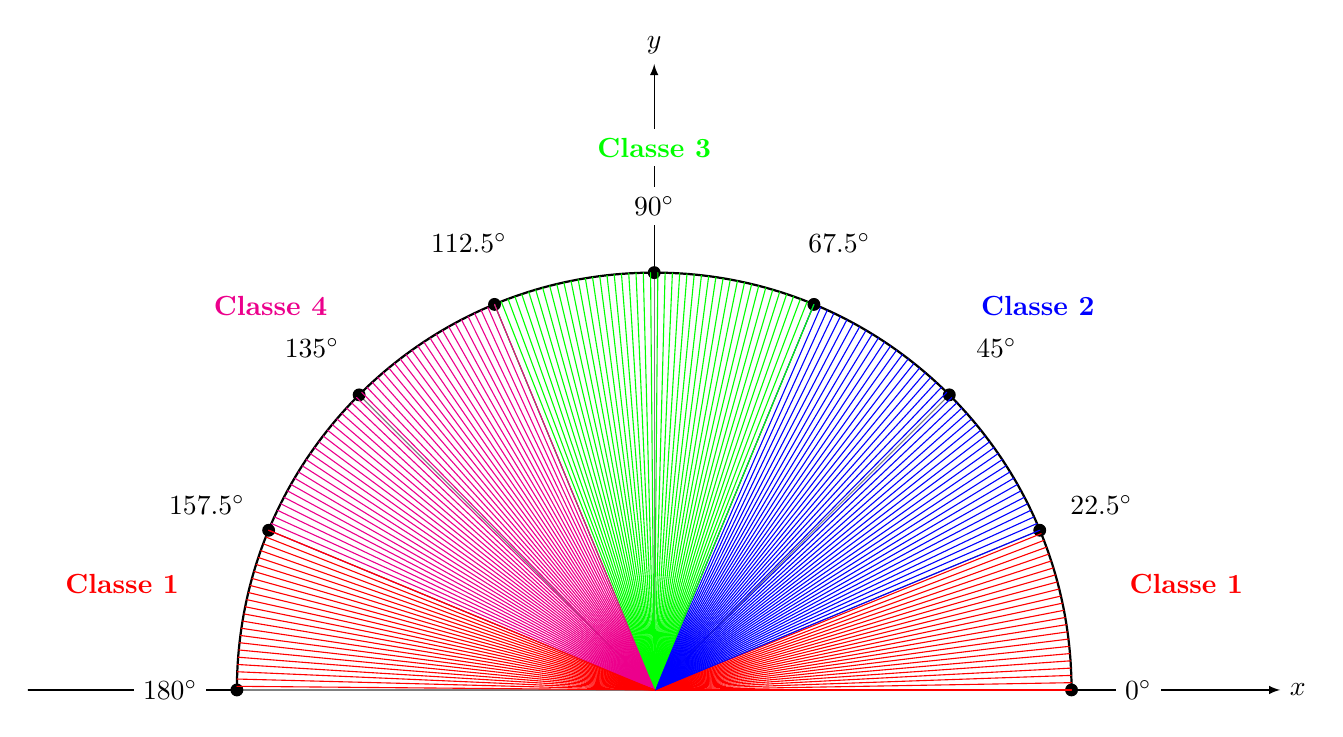
\begin{tikzpicture}[scale=5.3,cap=round,>=latex]
	% draw the coordinates
	\draw[->] (-1.5cm,0cm) -- (1.5cm,0cm) node[right,fill=white] {$x$};
	\draw[->] (0cm,0cm) -- (0cm,1.5cm) node[above,fill=white] {$y$};
	
	% draw the unit circle	
	\begin{scope}
		\clip (-1.5,0) rectangle (1.5,1.5);\clip (-1.5,0) rectangle (1.5,1.5);
		% clip permet d'avoir le demi-cercle
		\draw[thick] (0cm,0cm) circle(1cm);			
	\end{scope}
	
	\foreach \x in {0,22.5,...,180} {
		  % lines from center to point
		  \draw[gray] (0cm,0cm) -- (\x:1cm);
		  % dots at each point
		  \filldraw[black] (\x:1cm) circle(0.4pt);
		  % draw each angle in degrees
		  \draw (\x:1.16cm) node[fill=white] {$\x^\circ$};
	}
	
	\draw (11.25:1.3cm) node[fill=white] {\textcolor{red}{\textbf{Classe 1}}};	
	\draw (45:1.3cm) node[fill=white] {\textcolor{blue}{\textbf{Classe 2}}};
	\draw (90:1.3cm) node[fill=white] {\textcolor{green}{\textbf{Classe 3}}};
	\draw (135:1.3cm) node[fill=white] {\textcolor{magenta}{\textbf{Classe 4}}};
	\draw (168.75:1.3cm) node[fill=white] {\textcolor{red}{\textbf{Classe 1}}};
	
	\foreach \x in {0,1,...,22.5} {
	  % lines from center to point
	  \draw[red] (0cm,0cm) -- (\x:1cm);
	}
	
	\foreach \x in {22.5,23.5,...,67.5} {
	  % lines from center to point
	  \draw[blue] (0cm,0cm) -- (\x:1cm);
	}
	
	\foreach \x in {67.5,68.5,...,112.5} {
	  % lines from center to point
	  \draw[green] (0cm,0cm) -- (\x:1cm);
	}
	  
	\foreach \x in {112.5,113.5,...,157.5} {
	  % lines from center to point
	  \draw[magenta] (0cm,0cm) -- (\x:1cm);
	}
	
	\foreach \x in {157.5,158.5,...,180} {
	  % lines from center to point
	  \draw[red] (0cm,0cm) -- (\x:1cm);
	}
\end{tikzpicture}
\\\\
On traite ensuite les cas suivants : \\
\\
\textcolor{red}{\textbf{Classe 1}} (le contour est dans la direction Nord \--- Sud) : le pixel est un contour si la norme du gradient en ce point est supérieure au maximum de la norme du gradient des pixels Est et Ouest \\
\\
\textcolor{blue}{\textbf{Classe 2}} (le contour est dans la direction Nord-Ouest \--- Sud-Est) : le pixel est un contour si la norme du gradient en ce point est supérieure au maximum de la norme du gradient des pixels Nord-Est et Sud-Ouest \\
\\
\textcolor{green}{\textbf{Classe 3}} (le contour est dans la direction Est \--- Ouest) : le pixel est un contour si la norme du gradient en ce point est supérieure au maximum de la norme du gradient des pixels Nord et Sud \\
\\
\textcolor{magenta}{\textbf{Classe 4}} (le contour est dans la direction Nord-Est \--- Sud-Ouest) : le pixel est un contour si la norme du gradient en ce point est supérieure au maximum de la norme du gradient des pixels Nord-Ouest et Sud-Est \\
\\
Après cette étape, l'image n'est pas encore binarisée mais on a mis à 0 les pixels qui ne constituaient pas un contour.

\subsection{Etape 4/4 : Seuillage par hystérésis}

Le seuillage par hystérésis permet de retirer les faux contours. \\
\\
Pour cela, on définit deux seuils : 
\begin{itemize}
\item[•] \emph{Smin} : seuil minimum
\item[•] \emph{Smax} : seuil maximum \\
\end{itemize}

Pour chaque pixel de la norme du gradient obtenu après la suppression des non-maxima locaux, on regarde sa valeur. \\
\\
\textbf{Cas 1} : si la valeur du pixel est supérieure au seuil maximum alors ce pixel est un vrai contour donc on met sa valeur à 1 \\
\textbf{Cas 2} : si la valeur du pixel est inférieure au seuil minimum alors ce pixel est un faux contour donc on met sa valeur à 0 \\
\textbf{Cas 3} : si la valeur du pixel est entre le seuil minimum et le seuil maximum alors on regarde les valeurs des huit pixels voisins et on regarde s'il existe au moins un pixel voisin qui a une valeur supérieure au seuil maximum. Si c'est le cas, la valeur du pixel initial devient un 1 sinon 0 \\
\\
Pour le \textbf{Cas 3}, dans le code, on prend une fenêtre $3$x$3$ pour obtenir facilement les voisins du pixel au centre de cette fenêtre. \\

\begin{center}
\begin{tikzpicture}[scale=5.3,cap=round,>=latex]
        % draw the coordinates
        \draw (0.75,1.2) node[anchor=south] {\textbf{Vrai contour}};
        \draw[-] (-0.05cm,1cm) -- (1.5cm,1cm) node[right,fill=white] {\emph{Smax}};
        \draw (0.75,0.7) node[anchor=south] {\textbf{Contour incertain}};
        \draw[-] (-0.05cm,0.5cm) -- (1.5cm,0.5cm) node[right,fill=white] {\emph{Smin}};
        \draw (0.75,0.2) node[anchor=south] {\textbf{Faux contour}};
        \draw[-] (0cm,0cm) -- (1.5cm,0cm) node[right,fill=white] {};        
        \draw[->] node[below,fill=none] {$0$} (0cm,0cm) -- (0cm,1.5cm) node[above,fill=white] {$255$} ;
\end{tikzpicture}
\end{center}

L'image obtenue est maintenant binarisée. Elle contient les contours de l'image initiale et un peu de bruit.

\newpage
\section{Choix des hyper-paramètres}
\paragraph{}

	Le choix des hyper-paramètres pour le filtre de Kalman est particulièrement difficile. En effet, dans un cas réel, il est difficile de quantifier le bruit (covariance de l'état initial ($p_0$), bruit de transition ($Q$) et bruit d'observation ($R$)). Nous nous sommes donc basés sur les hyper-paramètres choisis dans la vidéo \href{https://fr.mathworks.com/videos/introduction-to-kalman-filters-for-object-tracking-79674.html}{MathWorks} ($5$min$27$s) qui traite \emph{singleball.mp4} avec un filtre de Kalman.

\begin{align*}
& p_0=100000 \cdot \begin{pmatrix}
	1 & 0 & 0 & 0 & 0 & 0 \\
	0 & 1 & 0 & 0 & 0 & 0 \\
	0 & 0 & 1 & 0 & 0 & 0 \\
	0 & 0 & 0 & 1 & 0 & 0 \\
	0 & 0 & 0 & 0 & 1 & 0 \\
	0 & 0 & 0 & 0 & 0 & 1 \\
\end{pmatrix} \quad
& Q=100000 \cdot \begin{pmatrix}
	25 & 0 & 0 & 0 & 0 & 0 \\
	0 & 25 & 0 & 0 & 0 & 0 \\
	0 & 0 & 10 & 0 & 0 & 0 \\
	0 & 0 & 0 & 10 & 0 & 0 \\
	0 & 0 & 0 & 0 & 1 & 0 \\
	0 & 0 & 0 & 0 & 0 & 1 \\
\end{pmatrix} \quad
& R=\begin{pmatrix}
	25 & 0 \\
	0 & 25 \\
\end{pmatrix}
\end{align*}

	Nous avons rencontré un problème lors de la définition de la matrice de transition $A$.
	
\[A=\begin{pmatrix}
	1 & 0 & dt & 0 & 0 & 0 \\
	0 & 1 & 0 & dt & 0 & 0 \\
	0 & 0 & 1 & 0 & dt & 0 \\
	0 & 0 & 0 & 1 & 0 & dt \\
	0 & 0 & 0 & 0 & 1 & 0 \\
	0 & 0 & 0 & 0 & 0 & 1 \\
\end{pmatrix}\]

	Pour la vidéo \emph{singleball.mp4} par exemple, une des caractéristiques de cette vidéo était $ 30 \; images/seconde $. Nous pensions alors que $ dt = 1/30 \; s $ mais cela donnait des résultats erronés. Nous avons alors mis $ dt = 1 \; s $ et les résultats étaient satisfaisants. Finalement, nous avons choisi $ dt = 1.2 \; s $. Malheureusement, nous ne comprenons pas pourquoi cette valeur de $ dt $ permet de mieux paramétrer le filtre.


\newpage
\section{Résultats et interprétations \--- singleball.mp4}
\subsection{Résultats avec $ dt = 1.2 \; s $}

\begin{figure}[H]
\caption{Positions successives de la balle \--- Image 1 de la vidéo}
\centerline{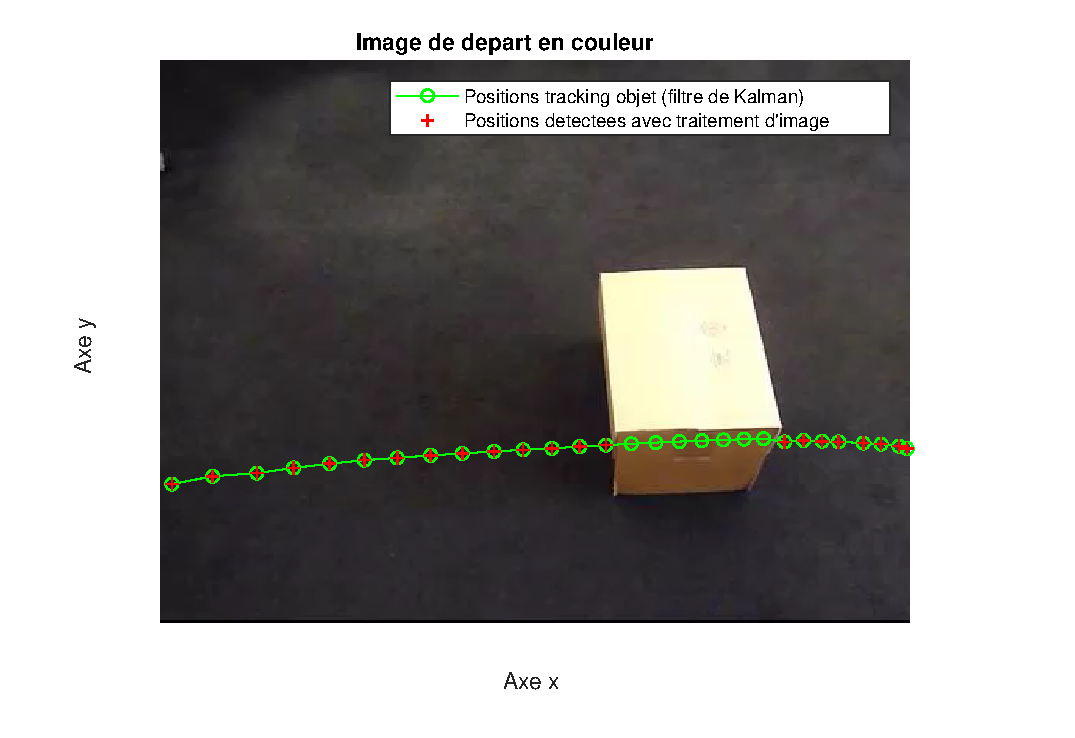
\includegraphics[width=20cm]{Images/Resultats/ImageDeDepartEnCourleur}}
\label{1}
\end{figure}

Sur la figure \ref{1}, les corrections des positions détectées semblent cohérentes. On remarque également que les prédictions des positions de la balle lorsqu'elle n'est pas détectée sont cohérentes.

\begin{figure}[H]
\caption{Positions successives de la balle}
\centerline{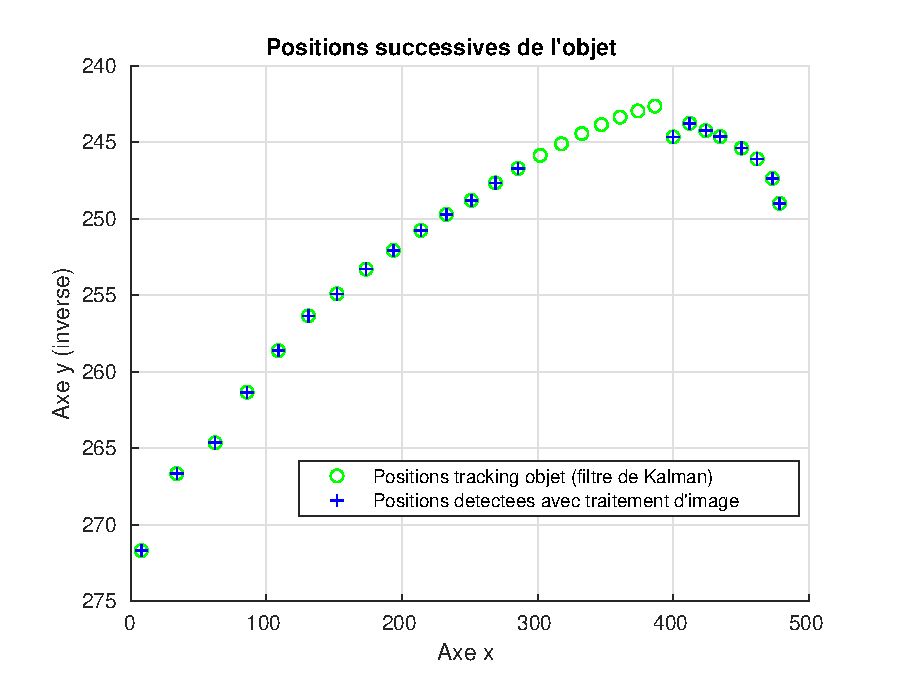
\includegraphics[width=20cm]{Images/Resultats/PositionsSuccessivesDeLObjet}}
\label{2}
\end{figure}

Sur la figure \ref{2}, on peut oberserver avec plus de détail les positions de la balle. On remarque que la prédiction des positions de la balle lorsqu'elle n'est pas détectée s'éloigne de sa vraie position. En effet, au bout de la septième prédiction, on voit que ce point est un peu éloigné de la position détectée lorsque la balle sort de l'autre côté de la boîte.

\subsection{Résultats avec $ dt = 1/30 \; s $ et ajustements de la vitesse et de l'accélération}

\begin{figure}[H]
\caption{Positions successives de la balle \--- Image 1 de la vidéo}
\centerline{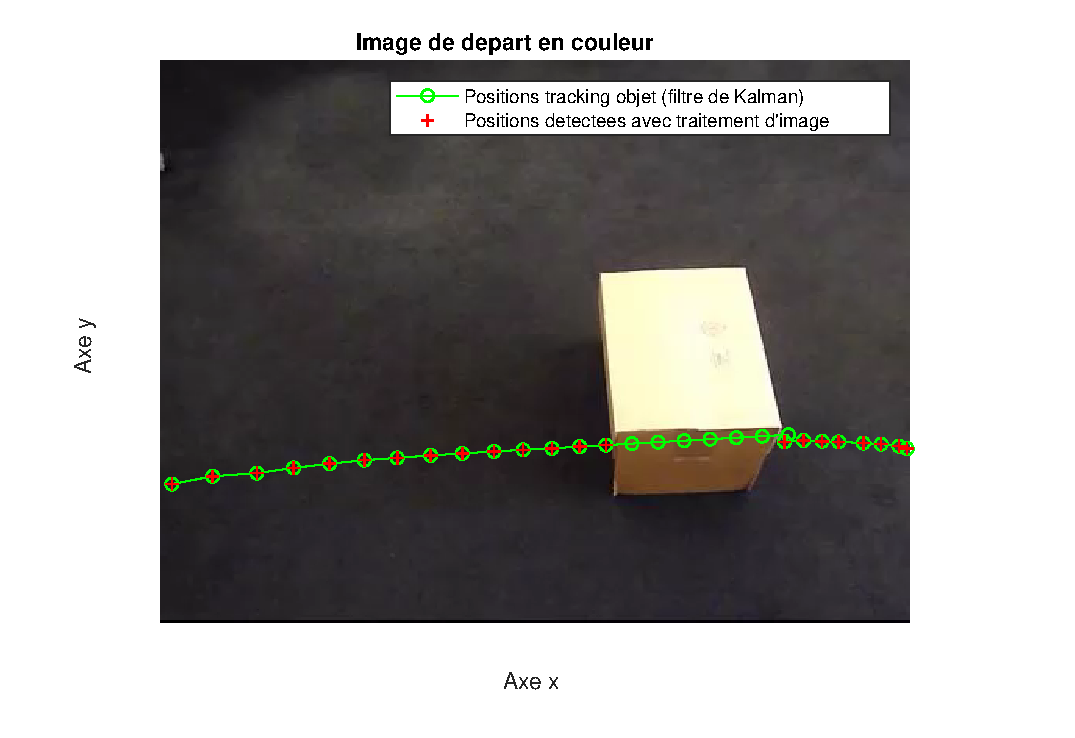
\includegraphics[width=20cm]{Images/Resultats/ImageDeDepartEnCourleur2}}
\label{3}
\end{figure}

Sur la figure \ref{3}, on remarque un problème lorsqu'on prédit la position de la balle quand elle n'est pas détectée. En effet, à la sortie de la boîte, le point prédit est trop loin.

\begin{figure}[H]
\caption{Positions successives de la balle}
\centerline{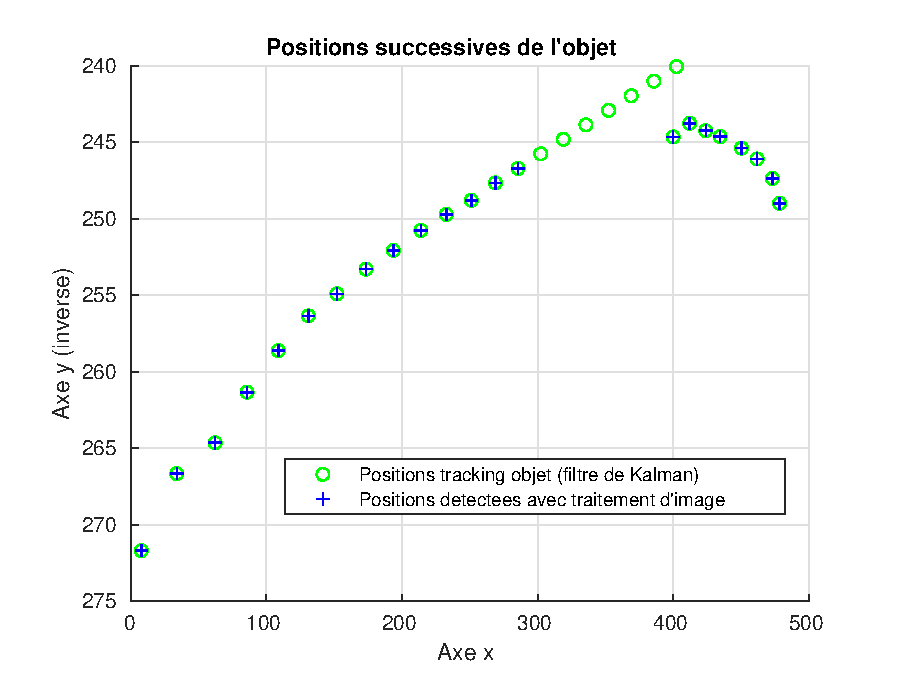
\includegraphics[width=20cm]{Images/Resultats/PositionsSuccessivesDeLObjet2}}
\label{4}
\end{figure}

Sur la figure \ref{4}, on remarque que les prédictions de la position de la balle quand elle n'est pas détectée ne sont pas bonnes. En effet, ces sept points ont une tendance linéaire et le septième point est éloigné du point détecté à la sortie de la boîte.






\newpage
\section{Bibliographie}
\begin{itemize}

\item[•] \textbf{\textcolor{magenta}{Article}}
\item[\textbf{Titre}] Using Canny's Criteria to Derive a Recursively Implemented Optimal Edge
Detector
\item[\textbf{Auteur}] RACHID DERICHE
\item[]

\item[•] Deriche edge detector
\item[] \url{https://en.wikipedia.org/wiki/Deriche_edge_detector} 

\item[•] Can't get clean output in my MATLAB implementation of Canny-Deriche
\item[] \url{https://stackoverflow.com/questions/14132356/cant-get-clean-output-in-my-matlab-implementation-of-canny-deriche} 

\item[•] Canny edge detector
\item[] \url{https://en.wikipedia.org/wiki/Canny_edge_detector} 

\item[•] Canny Edge Detection Step by step
\item[] \url{https://opencv-python-tutroals.readthedocs.io/en/latest/py_tutorials/py_imgproc/py_canny/py_canny.html} 

\item[•] Détection de contours : les opérateurs de Canny-Deriche
\item[] \url{https://perso.esiee.fr/~coupriem/Algo/algoima.html} 

\item[•] Extraction de contours et son extension du contour actif
\item[]
\url{http://ninebill.free.fr/ExtractionContours/detection/canny.html}

\item[•] JAVA demo of Canny/Deriche-like filter (EPFL Biomedical Imaging Group)
\item[] \url{http://bigwww.epfl.ch/demo/ip/demos/edgeDetector/} 

\item[•] Segmentator \--- Fix gramag export error with deriche filter (3D python)
\item[] \url{https://github.com/ofgulban/segmentator} 

\item[•] Edge Detection with MATLAB
\item[] \url{https://fr.mathworks.com/videos/edge-detection-with-matlab-119353.html} 

\item[•] Gaël Deest (pdf)
\item[] \url{www.theses.fr/2017REN1S102/abes} 

\item[•] Canny en python (OpenCV)
\item[] \url{https://opencv-python-tutroals.readthedocs.io/en/latest/py_tutorials/py_imgproc/py_canny/py_canny.html} 

\item[•] Convolution in Two Dimensions
\item[] \url{http://homepages.inf.ed.ac.uk/rbf/CVonline/LOCAL_COPIES/MARBLE/low/space/convol.htm} 

\item[•] Convolution en 2D
\item[] \url{http://web.stanford.edu/group/sequoia/cgi-bin/node/185} 

\item[•] EECS 442 \--- Computer vision
\item[] \url{http://vhosts.eecs.umich.edu/vision//teaching/EECS442_2012/lectures/lecture14.pdf} 

\item[•] DETECTION DE CONTOURS
\item[] \url{http://www.lirmm.fr/~strauss/PageImage3/EdgeDetection.pdf}

\item[•] Techniques d’extraction de contours
\item[] \url{ftp://ftp-sop.inria.fr/athena/Team/Rachid.Deriche/Lectures/Master-Stic-IGMMV/techniques_contours.pdf}

\item[•] Détection de contours
\item[] \url{http://devernay.free.fr/cours/vision/pdf/c3.pdf}

\item[•] Bases du traitement des images - Détection de contours
\item[] \url{http://webia.lip6.fr/~thomen/Teaching/BIMA/cours/contours.pdf}

\item[•] La détection decontours dans des images à niveaux de gris : mise en œuvre et sélection de détecteurs 
\item[] \url{http://docnum.univ-lorraine.fr/public/INPL_T_1991_ZIOU_D.pdf}

\item[•] Detection de contours
\item[] \url{http://dept-info.labri.fr/~achille/enseignement/TI/TI-ch4-notes.pdf}

\item[•] Segmentation d'image : Contours
\item[] \url{http://www.lgi2p.mines-ales.fr/~montesin/CoursPDF/segmentation_contours.pdf}

\item[•] Filtre de Deriche
\item[] \url{http://www.tsi.enst.fr/pages/enseignement/ressources/mti/Shen_ou_Deriche/node4.html}

\end{itemize}


\newpage
\section{Annexes}
\subsection{ProjetTSA.m}

\lstset{caption=ProjetTSA.m}
\lstinputlisting{../Code/ProjetTSA.m}

\subsection{trackingObjet.m}

\lstset{caption=trackingObjet.m}
\lstinputlisting{../Code/trackingObjet.m}

\subsection{kalmanFilter.m}

\lstset{caption=kalmanFilter.m}
\lstinputlisting{../Code/kalmanFilter.m}

\subsection{kalmanFilterAjustementsVitesseAcceleration.m}

\lstset{caption=kalmanFilterAjustementsVitesseAcceleration.m}
\lstinputlisting{../Code/kalmanFilterAjustementsVitesseAcceleration.m}

\subsection{kalmanFilterForTracking.m}

\lstset{caption=kalmanFilterForTracking.m}
\lstinputlisting{../Code/kalmanFilterForTracking.m}

\end{document}

